\section{A Closer Look at Non-linearity in Adam}
\label{sec:motivation}
\begin{figure*}[t!]
  \centering
  \subfigure[$\|\*v_t-\*v_{t-1}\|$]{
  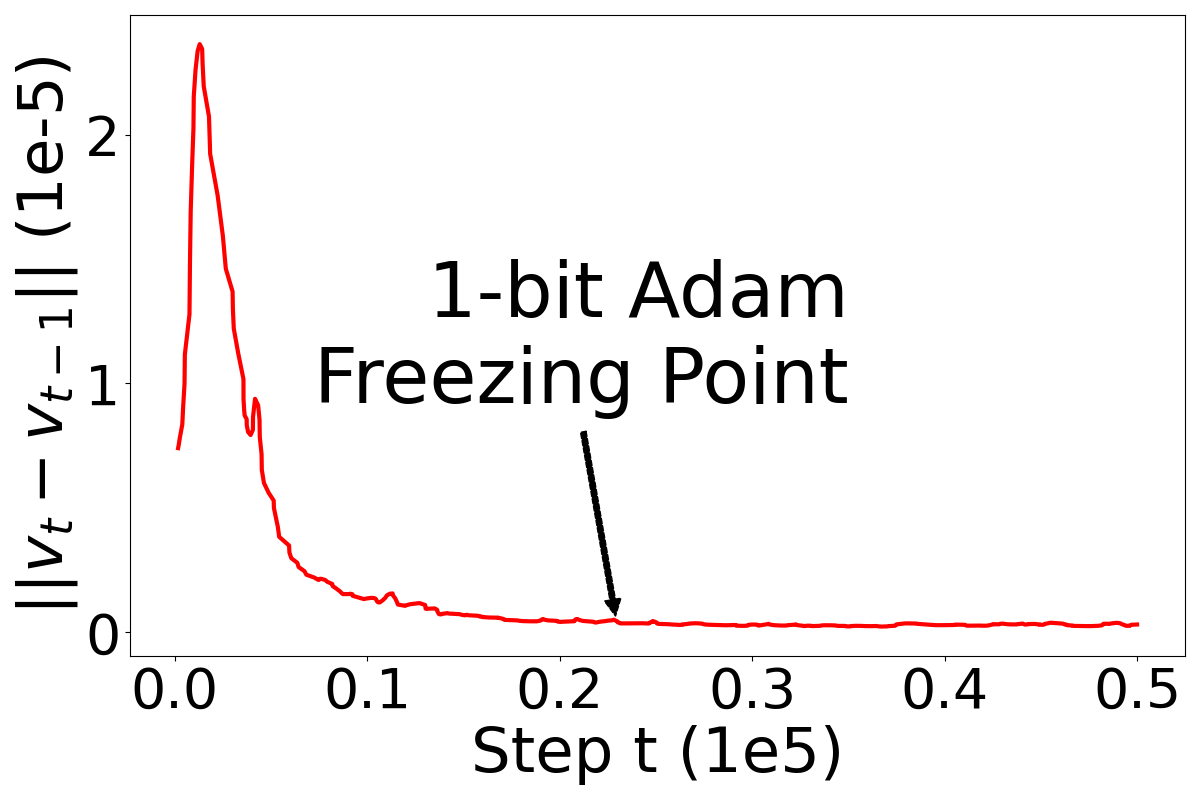
\includegraphics[width=0.23\textwidth]{./sections/figure/v_diff.png}\label{fig:profile_bert_large:var_diff_time}}
  \subfigure[$\|\*v_t^{(0)}-\*v_t\|$]{
  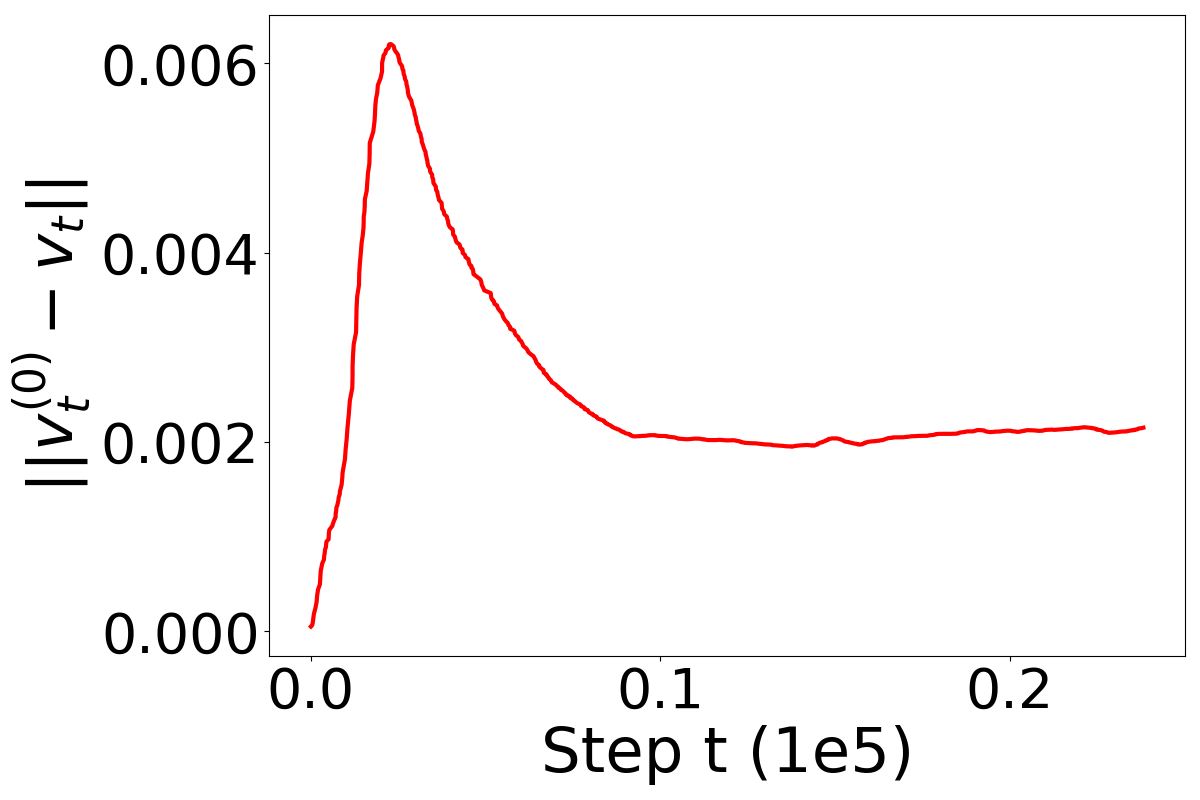
\includegraphics[width=0.23\textwidth]{./sections/figure/v_diff_local.png}\label{fig:profile_bert_large:var_diff_local}}
  \subfigure[$\|\*m_t-\*m_{t-1}\|$]{
  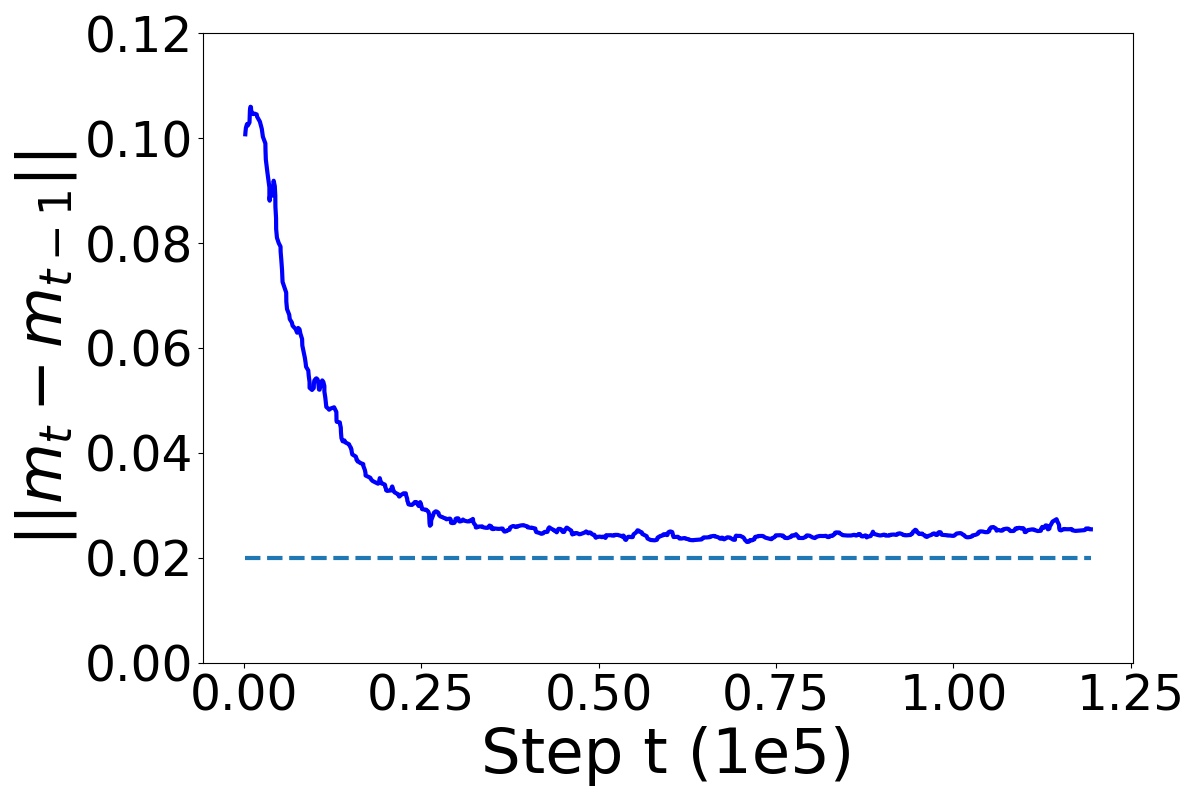
\includegraphics[width=0.23\textwidth]{./sections/figure/m_diff.png}\label{fig:profile_bert_large:mom_diff_time}}
  \subfigure[$\|\*m_t^{(0)}-\*m_t\|$]{
  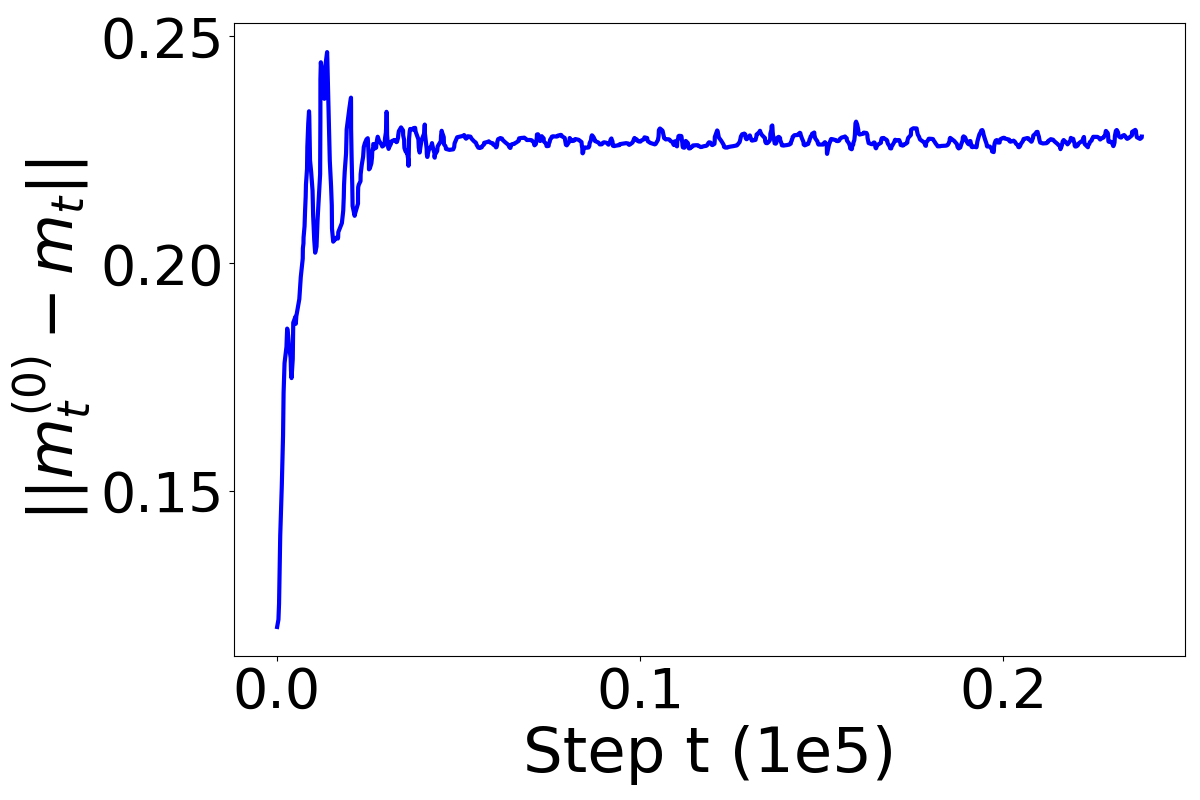
\includegraphics[width=0.23\textwidth]{./sections/figure/m_diff_local.png}\label{fig:profile_bert_large:mom_diff_local}}
  \caption{Momentum and variance Profiling for BERT-Large sequence 128 pretraining with original Adam using 64 GPUs. For variance, we profile two types of metrics: the first is the difference between local and global variance: $\|\*v_t^{(0)}-\*v_t\|$, where $\*v_t^{(0)}$ and $\*v_t$ denotes the variance term computed via local gradient on worker-0 and the gradient from full-precision AllReduce, respectively. We also profile the variance difference in adjacent step $\|\*v_t-\*v_{t-1}\|$. Similarly, we profile the same two metrics for the momentum.}
  \label{fig:profile_bert_large}
\end{figure*}

In this section, we provide a more formal description on the problem setting and illustrate the limitations from the original Adam and the state-of-the-art 1-bit Adam \citep{tang20211}.

\textbf{Problem Formulation.}
In this paper, we consider the following optimization problem:
\begin{align}
    \min_{\*x\in\mathbb{R}^d}f(\*x) = \mathbb{E}_{\zeta\sim\mathcal{D}}f(\*x;\zeta).
\end{align}
where $\*x$ denotes the $d$-dimensional model. $\mathcal{D}$ denotes the training set and $f(\*x;\zeta)$ is the loss incurred over sample $\zeta$ given model parameters $\*x$.
The structure of the problem naturally captures many of the model training problems.

\textbf{The non-linearity in Adam.}
At step $t\geq 0$, denote $\*x_t$ and $\*g_t$ as the model parameters and stochastic gradient computed at step $t$, respectively. The update formula of SGD and Adam\footnote{Note that in Adam, operations like division should act element-wise.} can be summarized as:
\begin{align}
\label{equa:SGD_update}
\text{SGD update: } & \*x_{t+1} \leftarrow \*x_t - \gamma \*g_t. \\
\text{Adam update: } & \*m_{t+1} \leftarrow \beta_1\*m_{t} + (1-\beta_1)\*g_t, \nonumber \\
& \*v_{t+1} \leftarrow \beta_2\*v_{t} + (1-\beta_2)(\*g_t)^2, \nonumber \\
    \label{equa:Adam_update}
    & \*x_{t+1} \leftarrow \*x_t - \underbrace{\frac{\gamma}{\sqrt{\*v_t + \epsilon}}}_{\text{effective learning rate}} \cdot \*m_t,
\end{align}
where $\gamma$ is the learning rate, $\epsilon$ is a small constant to prevent zero division, $\beta_1$ and $\beta_2$ are tunable decaying factors.
The linearity in SGD update implies when using compression or local steps, the potential noise from (accumulated) gradients is in the order of $O(\gamma)$, which approaches zero when learning rate is decaying or set to be small. By comparison, the two auxiliary optimizer states in Adam, momentum ($\*m$) and variance ($\*v$), introduce non-linearity in the model update. 

Equation~(\ref{equa:Adam_update}) gives the formula of Adam when running it sequentially. In a distributed setting with $n$ workers, $\*g_t$ in Equation~(\ref{equa:Adam_update}) is often computed in parallel on different workers. Mathematically, if we denote $\*g_t^{(i)}$ as the stochastic gradient computed on the $i$-th worker at step $t$, then distributed Adam can be written as replacing $\*g_t$ with $1/n\sum_{i=1}^n{\*g_t^{(i)}}$ in Equation~(\ref{equa:Adam_update}) as follows:
\begin{align*}
\*m_{t+1} \leftarrow \beta_1\*m_{t} + (1-\beta_1)\left(1/n\sum\nolimits_{i=1}^n{\*g_t^{(i)}}\right), \hspace{1mm} \*v_{t+1} \leftarrow \beta_2\*v_{t} + (1-\beta_2)\left(1/n\sum\nolimits_{i=1}^n{\*g_t^{(i)}}\right)^2.
\end{align*}
% This non-linearity brings up two limitations: 1) when aggressively compressing the gradient such as with 1-bit quantizer, all the coordinate-wise effect learning rate $\gamma/\sqrt{\*v_t+\epsilon}$ will become the same value, so that Adam no longer enjoys adaptive and fast convergence; 2) to keep all parallel workers to have a consensus on the optimizer state ($\*m$ and $\*v$), which is an important property for convergence, the existence of non-linearity forces all the workers to perform synchronization when performing local steps. However, this would add expensive synchronization overhead


\textbf{Issue with non-linearity on 1-bit  compression.}
The main bottleneck in running distributed Adam is the accumulation of $1/n\sum\nolimits_{i=1}^{n}\*g_t^{(i)}$ since the gradients are usually high-dimensional. 
Based on the profiling results from \citep{tang20211,li20211}, the communication of gradients could take up to 94\% of the total training time on modern clusters.
Gradient compression mitigates this issue by sending and averaging gradients with fewer bits. However, in Adam this causes the loss on the learning rate adaptivity. Consider using the aggressive
1-bit compression \citep{liu2018signsgd}, which sends each gradient with only signs and a shared, usually the average over all the coordinates, magnitude. More specifically, denote $\mathcal{C}[\cdot]$ as the 1-bit compression, then
\begin{align}
\label{equa:1bitcompression}
    \mathcal{C}[\*a] = \frac{\|\*a\|_1}{d} \cdot \text{sign}(\*a), \forall \*a\in\mathbb{R}^d.
\end{align}
It is straightforward to observe that naively applying 1 bit to compress gradients in the original Adam loses coordinate-wise adaptivity since sharing magnitude makes all the coordinates-wise learning rate $\gamma/\sqrt{\*v_t+\epsilon}$ the same value. This makes Adam no difference than momentum SGD.

\textbf{Issue with non-linearity on local steps.}
In SGD (Equation~(\ref{equa:SGD_update})), the model updates are linearly dependent on the gradients and has zero additional states. It implies with local steps, the parallel workers can entirely reach consensus after a single round of synchronization, even with compression \citep{basu2020qsparse}. However, in Adam simply synchronizing the model can still leave the momentum and variance out-of-sync. This makes parallel workers fail to capture the global adaptivity when the system scales up.
To give a more concrete example, we profile a full run of BERT-Large pre-training with original Adam, and summarize different metrics of momentum and variance in Figure~\ref{fig:profile_bert_large}. As shown in Figure~\ref{fig:profile_bert_large:mom_diff_local} and \ref{fig:profile_bert_large:var_diff_local}, the difference between local and global optimizer states, momentum and variance, remain constants and do not decrease to zero.

\textbf{1-bit Adam and its limitations.}
1-bit Adam \citep{tang20211} is a state-of-the-art solution that addresses non-linearity in 1-bit compression. 1-bit Adam adopts a pre-conditioned variance state from running original Adam for $T_0$ steps first. 
% Note that here we defer the details of 1-bit compression to Appendix~\ref{appendix:sec:algorithm} and treat it as a black-box procedure named \textbf{1bit-AllReduce} while the original full-precision AllReduce is referred to as \textbf{AllReduce}. 
The intuition there is that at later stage of training, the variance state becomes stable so that $\*v_{T_0}$ can be a good approximation of variance state for the remaining steps. 
As paritally illustrated in Section~\ref{sec:intro}, the full-precision stage of 1-bit Adam still presents non-trivial overhead. For instance: as illustrated in \citep{tang20211}, when training BERT-Large on 64 GPUs using Ethernet, while the full-precision stage contains 15\% of the total steps, it can take more than 50\% of the entire training in terms of the wall-clock time\footnote{Concretely, it shows in \citep{tang20211} Section 7.1 that to train BERT-Large on 64 GPUs using Ethernet, the full-precision Adam takes 174.3 hours in total while 1-bit Adam takes 51.5 hours. By a simple calculation, we know that full-precision stage of 1-bit Adam takes approximately 26.37 hours while the compression stage takes 25.13 hours.}.
Additionally, 1-bit Adam is restricted in the scope of compression, how it handles other techniques such as local steps remains open question.
% Additionally, we profile the per-step time for BERT-Large pretraining on a Ethernet cluster\footnote{The detailed profiling numbers can be found in Appendix~\ref{appendix:sec:experiment}.} and observe in a single step, the fixed cost of communication can take up to 4$\times$ of the computation time. This implies when data volume per-parameter reaches its extreme in training large models at large scales, the fixed cost of communication and compression could gradually become the bottleneck that dominates the computation time.

